\chapter{Reliability Analysis}
\chaptermark{Reliability}

The attempt to define the difference between \emph{reliability} and \emph{quality} will certainly fail, since given the intentional ambiguity in our definition of quality (Chapter~\ref{sec:introduction}).
For our purposes, however, this terminological matter will not matter, since we will simply define reliability analysis to be the analysis of the \emph{time} to \emph{failure}.
We will also assume that ``time'' and ``failure'' are well defined and agreed upon.

We intuitively understand ``more reliable'' to mean ``lasts longer''. 
We should also consider, however, the case of a product that is designed to fail after some time, thus forcing the consumer to buy a new one. 
Some may say that a major hi-tech company named after a fruit employs this practice. 
Be it true or not, I hope we can agree that good knowledge of your product's life expectancy is a desirable. 

Reliability analysis involves the study of a probabilistic property of our product- its \emph{survival}.
Any probabilistic model will require calibration to reality via data. 
This chapter thus introduces both the probability calculus typically used for reliability analysis, and some statistical considerations involved when calibrating these models.



\section{Probabilistic Analysis}




\subsection{A Static View}

Let $\x_j \in \set{0,1}, j=1,\dots,p$ denote the state of the $j$'th component of a system, and $x=(x_1,\dots,x_p)$.

\begin{definition}[Structure Function]
The \emph{structure function}, $\struct=\struct(x):x \mapsto \set{0,1}$, is an indicator function of the state of the system. A failure indicated by $0$. 
\end{definition}

\begin{remark}[$\Phi$]
We apologize to the reader for using $\Phi$ to denote both the $\gauss{0,1}$ CDF, and the structure function.
We do so to stay in accordance with reliability literature, and since no collisions are created in this chapter by doing so.
\end{remark}

\begin{definition}[Series System]
A \emph{series system}, or \emph{serial system}, is one where all components need to function for the system to function: $$\struct(x)=\prod_{j=1}^{p}x_j.$$
\end{definition}
A reliability diagram of a series system is given in Figure~\ref{fig:series_system}.
\begin{figure}[ht]
\centering
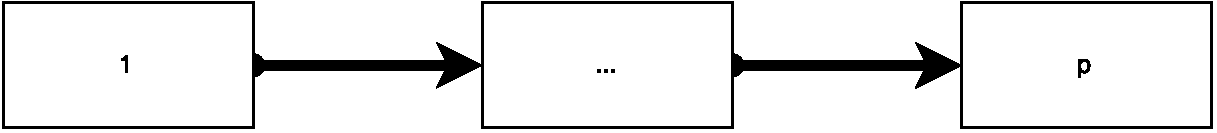
\includegraphics[width=0.5\linewidth]{art/series_system}
\caption{Series system.}
\label{fig:series_system}
\end{figure}


\begin{definition}[Parallel System]
A \emph{parallel system} is one where all components need to fail for the system to fail:
$$\struct(x)=1-\prod_{j=1}^{p} (1-x_j)= \coprod_{j=1}^p x_j.$$
\end{definition}
A reliability diagram of a parallel system is given in Figure~\ref{fig:parallel_system}.
\begin{figure}[ht]
\centering
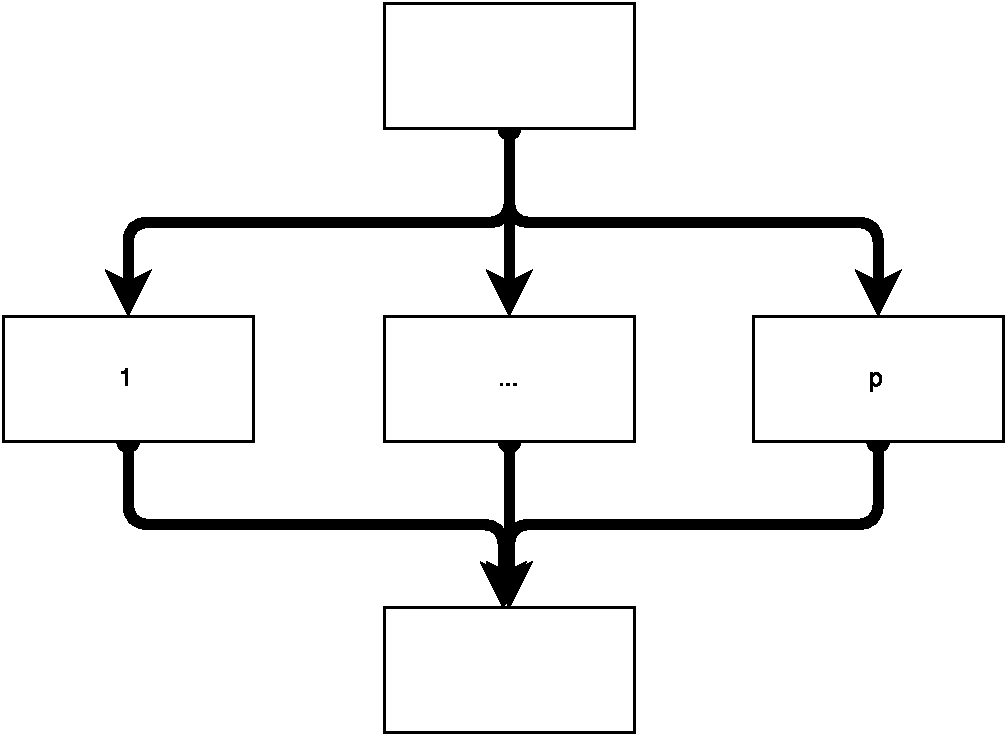
\includegraphics[width=0.5\linewidth]{art/parallel_system}
\caption{Parallel system.}
\label{fig:parallel_system}
\end{figure}


\begin{definition}[k-out-of-p System]
A \emph{k-out-of-p} system is one where at least $k+1$ components need to fail for the system to fail:
$$\struct(x)=\indicator{\sum_{j=1}^{p} x_j \geq k}.$$
\end{definition}
A reliability diagram of a k-out-of-p system is not provided, since it is not very friendly.




\begin{definition}[Monotone System]
A system is said to be \emph{monotone} if $\struct(x_1,\dots,x_p)$ is non decreasing in all components.
\end{definition}
The definition of monotonicity captures the idea that you cannot improve a system's state by breaking components.
This seems rather natural (I am still looking for a counter example).






\begin{definition}[Reliability]
We define the \emph{reliabity of component $j$} to be $$p_j:= P(\x_j=1),$$ 
and  the \emph{reliability of the system} 
$$ S_\struct:=P(\struct(x)=1).$$
\end{definition}


\begin{example}[Reliability of a series system]
For $\Phi(x)$ a series system, assuming independent components, we have
$$ S_\struct= \prod_{j=1}^{p} p_j.$$
\end{example}


\begin{example}[Reliability of a parallel system]
For $\Phi(x)$ a parallel system, assuming independent components, we have
$$ S_\struct= 1-\prod_{j=1}^{p} (1-p_j)= \coprod_{j=1}^p p_j. $$
\end{example}


\begin{example}[Reliability of a k-out-of-p system]
For $\Phi(x)$ a k-out-of-p system, assuming independent components with equal reliability ($p_i=p$), we have
$$ S_\struct= \sum_{i=k}^{p} \binom{n}{i} p^i (1-p)^{n-i} .$$
\end{example}



\subsubsection{State enumeration method}
To compute the reliability of more complex structures, one may use the state \emph{state enumeration method}. 
This method simply relies on summation of the probabilities of the states for which the system functions.
$$ S_\struct= \sum_{x} \Phi(x) P(\x=x).$$


\subsubsection{Factoring method}
The \emph{factoring method}, \aka \emph{pivot-decomposition method}, relies on two ingredients: 
(a) conditioning on the state of some components greatly simplifies the structure, and
(b) the total probability argument.
Combining the two we have:
$$ S_\struct= p_j  S_{\struct|x_j=1} + (1-p_j) S_{\struct|x_j=0}   .$$
The following example demonstrates the power of the factoring method.

\begin{example}[Bridge Structure]
\label{eg:bridge}
Consider structure in Figure~\ref{fig:bridge}.
To compute the reliability, we will call upon the factoring method while conditioning on the state of component $3$:
$$ S_\struct= p_3  S_{\struct|x_3=1} + (1-p_3) S_{\struct|x_3=0}   .$$
Now note that when $x_3=1$ then we have a series structure of parallel structures, while when $x_3=0$ we have a parallel structure of series structures.:
\begin{align*}
	S_{\struct|x_3=1} &= (p_1 \coprod p_2) (p_4 \coprod p_5)\\
	S_{\struct|x_3=0} &=  p_1 p_4 \coprod p_2 p_5 \\
	S_\struct &= p_3  (p_1 \coprod p_2) (p_4 \coprod p_5) + (1-p_3) (p_1 p_4 \coprod p_2 p_5).
\end{align*}

\begin{figure}[ht]
\centering
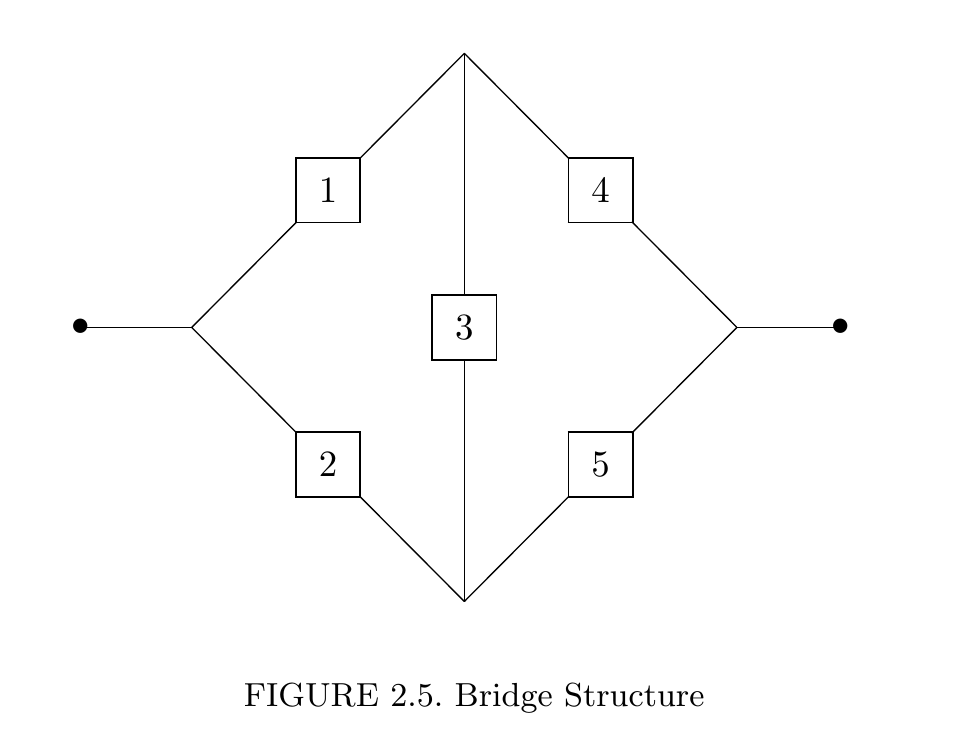
\includegraphics[width=0.5\linewidth]{art/bridge}
\caption{Structure of a bridge system. Source: \cite[Fig.2.5]{aven_stochastic_1999}}
\label{fig:bridge}
\end{figure}

\end{example}
Example~\ref{eg:bridge} demonstrates a single application of the factoring method. Clearly, it can be applied recursively for more complicated systems.

The example also demonstrates a more general principle. Namely, that redundancy is preferable at the component level, and not at the system's level.
Put differently- when designing a backup, and the resources allow a fill copy of the original system, we are better of by designing a component-wise backup, than a single backup system.
Put formally:
\begin{theorem}[Component-wise redundancy]
For a monotone structure $\Phi$, 
\begin{align}
	S_{\struct(x \coprod y)} \geq S_{\struct(x)} \coprod S_{\struct(y)}
\end{align}
where $x \coprod y$ denotes a component-wise backup: $(x_1 \coprod y_1,\dots,x_p \coprod y_p)$.
\end{theorem}



\begin{extra}[Reliability analysis of complex systems]
Except for simple systems, of the type we presented, the computation of the reliability of a complex system may be a formidable task. 
For complicated real-life systems, \emph{min-cut--max-flow} algorithms, or \emph{inclusion-exclusion} type algorithms are employed. 
For more details, see \cite{aven_stochastic_1999}.
\end{extra}









\subsubsection{Reliability Importance Measures}
\begin{quotation}
The Strength Of The Chain Is In The Weakest Link.
\end{quotation}
This is obviously a profound observation in reliability analysis.
In order to identify the weakest link we require some measure of reliability importance.


\begin{definition}[Improvement potential]
The \emph{improvement potential} is defined as the change in a system's reliability, if we could force a component to function indefinitely.
Formally, we denote $\Phi^{(j)}$ to be a system where component $j$ cannot fail. 
We then define the improvement potential with respect to component $j$ to be 
\begin{align}
	I_j :=S_{\Phi^{(j)}}-S_{\Phi}.
\end{align}
\end{definition}



\begin{definition}[Birenbaum's measure]
\emph{Birenbaum's measure} is defined as the change in a system's reliability, if we infinitesimally improve the reliability of component $j$.
Formally 
\begin{align}
	I_j: =\frac{\partial}{\partial p_j} S_{\Phi}.
\end{align}
\end{definition}


Clearly any such importance measure, once computed, may serve to decide which component should be treated to improve reliability.







\subsection{A Time Dynamic View}
The reliability of each component ($p_j$), typically changes in time, and so does the reliability of the whole system.
In the following, $\T$ will typically stand for the time to malfunction. It is thus assumed to be \textbf{continuous} and \textbf{non-negative}.


\begin{definition}[CDF]
The cumulative distribution function (CDF) of a random variable $\T$ at a point $t$  is given by
\begin{align}
	\cdf{\T}{t}:= P(\T<t).
\end{align}
\end{definition}

\begin{definition}[PDF]
The probability density function (PDF) of a continuous random variable $\T$ at a point $t$ is given by 
\begin{align}
	\pdf{\T}{t}:= \frac{\partial}{\partial t}\cdf{\T}{t}.
\end{align}
\end{definition}


\begin{definition}[Survival Function]
The survival function of a random variable $\T$ at a point $t$ is given by 
\begin{align}
	\survive{\T}{t}:= P(\T>t)=1-\cdf{\T}{t}.
\end{align}
\end{definition}
By definition, it follows that if $\T_j$ is the time to failure of component $j$, then $p_j(t)=\survive{\T_j}{t}$.
If $\T_\struct$ is the time to failure of a system $\Phi$, then we may write $S_\struct(t)=\survive{\T_\struct}{t}$.


\begin{example}[Survival of a series system]
For a series system $\struct$, the reliability of the system at time $t$ is given by $$\survive{\Phi}{t}=\prod_{j=1}^{p} p_j(t).$$
\end{example}


\begin{example}[Survival of a parallel system]
For a parallel system $\struct$, the reliability of the system at time $t$ is given by $$\survive{\Phi}{t}=1- \prod_{j=1}^{p} (1-p_j(t))= \coprod_{j=1}^p p_j(t).$$
\end{example}





Another way to present a distribution, no less informative than the previous ones, is by the \emph{hazard function}, which is the ``probability of surviving just another instant''.
\begin{definition}[Failure Rate]
The \emph{hazard function}, or \emph{failure rate}, of a random variable $\T$ at a point $t$ is given by \marginnote{Hazard Function}
\begin{align}
	\hazard{\T}{t} &:= \lim_{dt\to 0}\frac{P( \T \in [t,t+dt)|\T \geq t )}{dt} \label{eq:hazard}\\
	&= \frac{\pdf{\T}{t}}{\survive{\T}{t}} \\
	&= \frac{\partial}{\partial t}\log \survive{\T}{t}.
\end{align}
\end{definition}





\begin{definition}[Cumulative Risk]
The \emph{cumulative hazard}, \aka the \emph{cumulative risk}, of a random variable $\T$ at a point $t$ is given by \marginnote{Cumulative Hazrd}
\begin{align}
	\cuhazard{\T}{t} &:= \int_{0}^{t}\hazard{\T}{t} \\
	\Rightarrow \survive{\T}{t} &= \exp(-\cuhazard{\T}{t}). \label{eq:cumhazrd}
\end{align}
\end{definition}
Eq.(\ref{eq:cumhazrd}) readily shows that a distribution is well defined by its hazards.



\begin{theorem}[Failure rate of a series system]
\label{thm:ifr_closure}
The failure rate of a series system of independent components $\Phi$ is given by the sum of the failure rates of its components
\begin{align}
	\hazard{\Phi}{t}= \sum_{j=1}^{p} \hazard{\T_j}{t}
\end{align}
\end{theorem}
The proof is immediate using the cumulative risk.
The failure rate of a parallel system, does not admit such a nice closed form as we will soon see in Example~\ref{eg:failure_parallel}.




\begin{example}[Exponential Hazard]
The simplest distribution when discussing hazards is the exponential.
Recalling
\begin{align}
	\pdf{\T}{t}= \lambda \exp(-\lambda t) \indicator{t \geq 0} \\
	\cdf{\T}{t}= (1-\exp(-\lambda t)) 
\end{align}
so that 
\begin{align}
	\survive{\T}{t} &= \exp(-\lambda t), \\
	\hazard{\T}{t} &= \lambda.
\end{align}
\end{example}
The exponential is the only distribution with constant hazard which makes it very easy to analyze.
The constant hazard is due to the \emph{memoryless} property. Look at Eq.(\ref{eq:hazard}) and think why.

% [HW: prove that memory less is sufficient]


\begin{example}[Failure rate of a series of exponential components]
The failure rate of a series system $\Phi$, of $p$ independent components each with exponentially distributed failure times, is simply 
\begin{align}
	\hazard{\Phi}{t}= \sum_{j=1}^{p} \lambda_j, \forall t \geq 0
\end{align}
where $\lambda_j=\lambda_j(t)$ is the rate of each component.
\end{example}
This is obviously the simplest system possible for reliability analysis, which stems from the fact that a minimum of exponentials is exponential with the sum of rates.



The following example, seemingly very simple, provides tremendous insight into the complexities of reliability analysis.
\begin{example}[Failure rate of a two exponential-component parallel-system]
\label{eg:failure_parallel}
Consider a system of two independent, parallel, exponential components, with failure times $\T_j\sim \exp(\lambda_j); j=1,2$.
The failure rate is given by
\begin{align}
	\hazard{\Phi}{t}=
	\frac
	{\exppdf{\lambda_1}{t} + \exppdf{\lambda_2}{t}  - \exppdf{(\lambda_1+ \lambda_2)}{t}}
	{\expcdf{\lambda_1}{t} + \expcdf{\lambda_2}{t} - \expcdf{(\lambda_1+ \lambda_2)}{t}}
\end{align}
\end{example}
Why is Example~\ref{eg:failure_parallel} so important?
Because it demonstrates that even in a simple system, with the simplest components, the reliability is not so simple to compute (as a function of the components' reliability). 
Indeed, even though the hazards are fixed, the system's hazard is non monotone in time (Figure~\ref{fig:hazard_non_monotone}). 


\begin{figure}[ht]
\centering
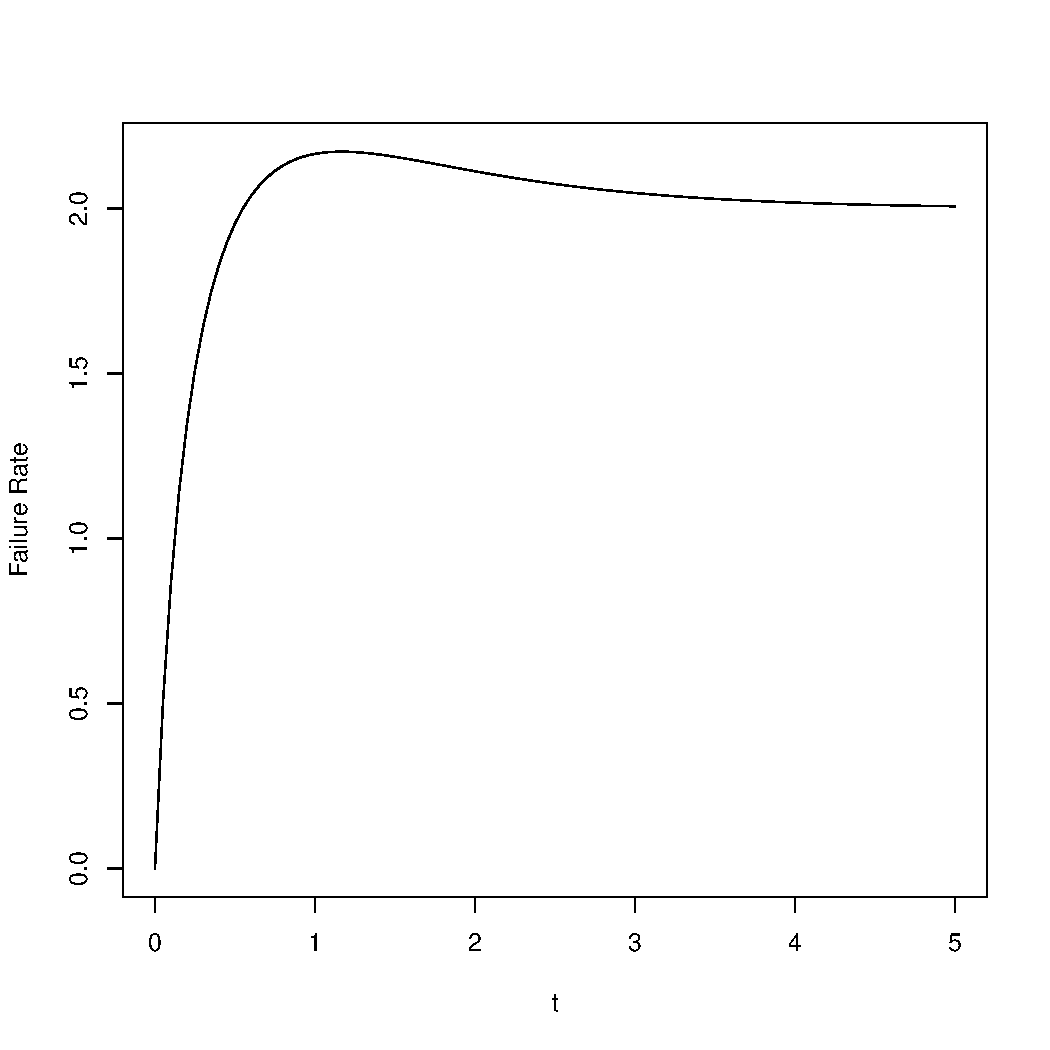
\includegraphics[width=0.5\linewidth]{art/hazard}
\caption{Failure rate of the parallel exponential component system.}
\label{fig:hazard_non_monotone}
\end{figure}





\begin{example}[Weibull Hazard]
The Weibull distribution is very common in reliability analysis, and can be constructed by 
$\T := \lambda \U^{1/k}$, where $\U \sim \exp(1)$. 
Recalling
\begin{align}
	\pdf{\T}{t} &= \frac{k}{\lambda}\left(\frac{\T}{\lambda} \right)^{k-1} \exp\left(-\frac{\T}{\lambda} \right)^k  \indicator{\T\geq 0} \\
	\cdf{\T}{t} &= 1 - \exp \left(-\frac{\T}{\lambda} \right)^k 
\end{align}
so that 
\begin{align}
	\survive{\T}{t} &= \exp \left(-\frac{\T}{\lambda} \right)^k \\
	\hazard{\T}{t} &= \frac{k}{\lambda} \left(\frac{\T}{\lambda} \right)^{k-1} .
\end{align}
\end{example}
Elementary analysis shows that the hazard function of the Weibull may be increasing or decreasing in time ($\T$), depending on $k$, but it is always monotone.




\begin{example}[Empirical risk rates]
When examining empirical risk rates of true devices, we almost always notice a \emph{bathtub} structure, such as in Figure~\ref{fig:bathtub}.\marginnote{Bathtub}
This shape captures the idea that products tend to fail more when they are brand new, or as they are very old, while their failure rates are fairly stable in the ``mid-life''.
In this text, we will not be providing a particular distribution which has this property. 
We refer the reader to \cite{nadarajah_bathtub-shaped_2008} for examples of distributions which have the bathtub property.
\end{example}


\begin{figure}[ht]
\centering
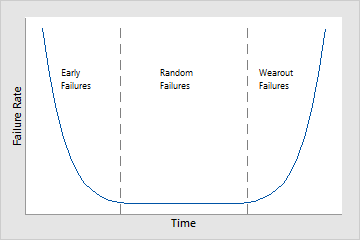
\includegraphics[width=0.5\linewidth]{art/bathtub_curve}
\caption[Bathtub empirical hazard curve]{Bathtub curve of empirical failure rates. \newline
\url{http://support.minitab.com/en-us/minitab/17/topic-library/modeling-statistics/reliability/distributions-in-reliability-analysis/hazard-functions/}}
\label{fig:bathtub}
\end{figure}




\subsubsection{Aging}
The idea of \emph{aging} is that failure rate may vary over time. It is an important concept in reliability, as demonstrated by the empirical bathtub failure rate (Figure~\ref{fig:bathtub}).
Instead of checking if a particular textbook distribution has some ageing property, we instead analyze classes of distributions with the desired notion of ageing.
Our goal will ultimately be to understand the ageing of a whole system, as a function of the ageing of its components.

\begin{definition}[IFR]
We call a failure time distribution to be in the \emph{increasing failure rate} (IFR) ageing class, if it has a non decreasing failure rate.
\end{definition}
We know from Example~\ref{eg:failure_parallel}, that two IFR components in parallel, are not an IFR system.


\begin{definition}[IFRA]
We call a failure time distribution to be in the \emph{increasing failure rate average} (IFRA) ageing class, if 
$\cuhazard{\T}{t}/t$ is non decreasing in $t$.
\end{definition}

\begin{definition}[NBU]
We call a failure time distribution to be in the \emph{new better then used} (NBU) ageing class, if 
$\survive{\T}{t_1+t_2} \leq \survive{\T}{t_2} \survive{\T}{t_1}$.
\end{definition}


\begin{definition}[NBUE]
Define the \emph{expected residual life}, $\mu(t)$, to be 
$$\mu(t):= \expect{\T-t|\T>t}.$$
\marginnote{Expected Residual Life}
We call a failure time distribution to be in the \emph{new better then used in expectation} (NBUE) ageing class, if 
$\mu(t) \leq \mu(0)$.
\end{definition}


\begin{theorem}
$IFR \Rightarrow IFRA \Rightarrow NBU \Rightarrow NBUE. $
\end{theorem}


The following theorem states a relation between the ageing properties of particular components, and that of the whole system. In particular it states that for the (very wide) class of monotone systems, then the IFRA property is conserved. 
This should be contrasted with the IFR property, which is not conserved, as demonstrated by Example~\ref{eg:failure_parallel}.
\begin{theorem}[IFRA closure theorem]
\label{thm:ifra_closure}
If the independent components of a monotone system are IFRA, then so is the whole system.
\end{theorem}


\begin{cor}[IFR closure for series systems]
\label{cor:ifr_series}
Series systems are a extremely small and particular subset of monotone systems.
It does provide, however, an example of systems where not only IFRA is preserved, but also the stronger IFR.
This statement follows immediately from Theorem~\ref{thm:ifr_closure} and the fact that a sum of monotone functions is monotone.
\end{cor}


\begin{extra}[IFR and log-concave]
The IFR requirement, is essentially the same as log-concavity of the density function.
This immediately implies many properties of the class.
See \cite{bagnoli_log-concave_2005}.
\end{extra}




Now consider a two-component system, where one component kicks-in when the first fails.
We will call this an \emph{offline backup}.\marginnote{Offline Backup}
The survival times of the components in an offline backup system are clearly dependent. 
It turns out that for such a system of IFR components, does conserve the IFR property, as seen in the following theorem.
\begin{theorem}[Convolution of IFR]
\label{thm:ifr_convolution}
For two independent random variables, $\x$ and $\y$, both in the IFR ageing class, then so is $\x+\y$.
\end{theorem}



\begin{example}[IFR of Gamma]
The Gamma (and thus the Erlang) distribution is in the IFR aging class, since it is the sum of exponentials, each with constant failure rates, thus each IFR.
\end{example}

\begin{example}[Series system of offline backups]
What can we say about the ageing class of a series systems of offline backup systems? 
It turns out that if the components are IFR, then so will the whole system.
This is immediate from Corollary~\ref{cor:ifr_series} and Theorem~\ref{thm:ifr_convolution}.
\end{example}






\section{Statistical Analysis}
The probabilistic analysis of the previous section is great fun and all, but like any probabilistic problem, is has to be calibrated to real life. 
This is where data, and statistics come in.
Indeed, given any particular probabilistic model, we may write the likelihood problem, and call upon maximum likelihood principles for estimation.

Failure data and models introduces particular statistical challenges:
\begin{description}
\item [Identifiability] It is typically hard, if not impossible, to estimate the reliability of particular components, from the reliability of the whole system. 
\item [Censoring] a major concern with reliability data, is that in any finite length experiment, some events will just not have happened yet; their failure time will thus be censored. Ironically- the more reliable a component, the less data we will have to estimate its reliability. 
\item [Lab versus real-life conditions] Reliable components take very long time to fail. We much rather extrapolate from harsh lab conditions to real-life operating conditions. This requires the introduction of covariates. 
\item [Failure Distribution] like any statistical model, we will need to commit to some failure time sampling distribution.
\end{description}


\subsection{Identifiability}

\begin{example}[Likelihood estimation of a series system]
\label{eg:likelihood_of_failures}
Assume a series system $\Phi$ with $p$ independent, exponential components with rates $(\lambda_1,\dots,\lambda_p)$.
We have $n$ observations on the failure times of the system $t_1,\dots,t_n$.
How can we estimate the failure rates?
To use a likelihood approach, we need the data's sampling distribution.
Denoting the failure time of the $j$'th component of the $i$th device with $\T_{i,j}$, we have that $\T_{i,j}\sim \exp(\lambda_j)$ by assumption.
Since the system is serial, then $\T_i=\min_j(\T_{i,1},\dots,\T_{i,p})$.
By the properties of the exponential distribution $\T_i \sim \exp(\lambda)$, where $\lambda:=\sum_{j=1}^{p} \lambda_j$, as we have already seen with the failure rate. It follows that
$\pdf{\T_i}{t}=\lambda \exp(-\lambda t)$.
We may then write the likelihood function, maximize it with respect to $\lambda$ and discover, as we already know, that $$\hat{\lambda}=\frac{n}{\sum_{i=1}^{n} t_i}.$$
We are now left with the problem of recovering $(\lambda_1,\dots,\lambda_p)$ from $\lambda$. 
Can we do it? On the face of it- no. Which should not surprise us, since the mere knowledge of a device failure, is not very informative on the particular component that failed, which we would need to estimate $(\lambda_1,\dots,\lambda_p)$.
\end{example}

Example~\ref{eg:likelihood_of_failures} teaches us that unless further assumptions are introduced, the estimation of the component-wise failure rates requires information on the component-wise failure times. 





\subsection{Censored Events}
Consider several components being analyze for their reliability. 
Ironically, we actually want them to fail. If they do not, they do not convey information on their reliability.
In the event that a component has not failed, we clearly cannot register its failure time. Omitting this component from the sample will upward bias the estimated reliability.
These events are called \emph{censored} observations. 
There are several types of censoring which depend on the design of the study and the type of event recorded. 
They are all dealt with careful though on the sampling distribution of the data, and the probability of a censoring event. 

Design considerations:
\begin{description}
\item [Type I] occurs when the design is such that the sampling time is fixed a-priori. This implies that the number of failures (thus censoring) events is random. 
\item [Type II] occurs when the design is such that the number of failures (thus censoring) is fixed a-priori. This implies that the sampling duration is random.
\end{description}
If all we know on a censored event is that the actual lifetime is larger then the observation period, we call this a \emph{non-informative} censoring. 
Both designs will then lead to the same modelling of the censoring event, which is now describe.

The likelihood function of non-censored events is given by
\begin{align}
	\lik_i=\density_\T(t_i)= \survive{\T}{t_i} \hazard{\T}{t_i},
\end{align}
and the likelihood of a censored event, under the \emph{non-informative} assumption, is given by 
\begin{align}
	\lik_i=\survive{\T}{t_i} .
\end{align}
Unifying the two cases assuming independent observations, using an indicator for censoring, $c_i$, and taking logs we have
\begin{align}
	\loglik &=\log \lik\\ 
	&= \log \prod_{i=1}^{n} \lik_i \\
	&= \log \prod_{i=1}^{n} \survive{\T}{t_i} \hazard{\T}{t_i}^{c_i} \\
	&= \sum_{i=1}^{n} [c_i \log \hazard{\T}{t_i} - \cuhazard{\T}{t_i}]. \label{eq:censored_likelihood}
\end{align}


\begin{example}[Censored exponential lifetimes]
Recalling that the failure rates of exponential lifetimes are fixed, we have that the likelihood of censored exponential lifetimes is given by 
$$
	\sum_{i=1}^{n} [c_i \log \lambda - \lambda t_i].
$$
The maximum likelihood estimator of $\lambda$ is thus
\begin{align}
	\estim{\lambda}= \frac{\sum c_i}{\sum t_i}. \label{eq:censored_ml}
\end{align}
Eq.(\ref{eq:censored_ml}) lends itself to a nice interpretation.
The nominator is the total number of failures.
The denominator is the total \emph{exposure time}. 
The estimated failure rate is thus the number of failures per unit of exposure time. 
\end{example}




\begin{extra}
The previous result is obvious is you consider failures as events which come as a Poisson process, which is implied from the exponential times assumption. 
The process is run for $\sum t_i$ time, and the total event count is $\sum c_i$. 
The trivial estimator for the rate of the process, is $\sum c_i/\sum t_i$.
\end{extra}






\subsection{Accelerated Life Models}
The \emph{accelerated life} model is very popular for very reliable components. This is because it may take forever to produce defect. We thus ``accelerate'' life, by testing under extreme conditions, and then scale back to the regular operating environments.

An accelerate life mode assumes that covariates rescale time. 
For instance, the lab may produce conditions where time advances ten times faster than in real-life operating conditions.
To introduce the model, we start with a simple two group example.
\begin{example}[Two group accelerated life]
Consider two groups indexed by a single dummy variable $x_i \in \set{0,1}$.
Assuming an accelerated life effect we have
$$
	\survive{x_i=1}{t}=\survive{x_i=0}{t/exp(\beta)}=\survive{x_i=0}{t/\gamma}, 
$$
where $\gamma$ is simply shorthand notation for $exp(\beta)$. 
If $\gamma=1/2$, this means that time for group $x_i=1$ advances twice as fast as for group $x_i=0$.
\end{example}

We now generalize the idea for multiple covariates.
If $\T_1$ is the time to failure under conditions $x_1$ , and $\T_2$ under conditions $x_2$. 
And the covariates' effects are such that $x_1' \beta=1$ and $x_2' \beta=\log \gamma$,  then 
\begin{align}
\label{eq:accelerated_life}
	\survive{\T_2}{t}=\survive{\T_1}{t/\gamma},
\end{align}
meaning that the conditions $x_2$ are such that time is accelerated by $1/\gamma$ compared to conditions $x_1$.


An equivalent formulation of an accelerated life model is the following:
\begin{align}
\label{eq:estimating_accelerated_life}
	\log \T_i = x_i'\beta + \varepsilon_i
\end{align}
for some error term $\varepsilon_i$. 
For the above interpretation, we again denote $x_i'\beta= \log \gamma_i$, and infer that $x_i$ accelerates time by $1/\gamma_i$. 
This formulation is more tractable for mathematical manipulation, but conceals the nice interpretation which motivates the model's name.

Eq.(\ref{eq:estimating_accelerated_life}) readily reveals how we can easily estimate the effects ($\beta$) of an accelerate life model.
We simply take the log of the survival times, and assuming the particular distribution of $\varepsilon$, we may estimate $\beta$ using maximum likelihood.



\begin{example}[Accelerated life with Gaussian noise]
\label{eg:accelerated_gaussian}
The maximum likelihood estimation of $\beta$ when assuming that $\varepsilon_i \sim \gauss{0,\sigma^2}$, collapses to a simple linear regression when the dependent variable is simply $\log t_i$.
\end{example}


\begin{extra}[Tobit regression]
Assuming $\varepsilon_i \sim \gauss{0,\sigma^2}$, as in the previous example, implies that failure times are \emph{log normal} distributed. 
This approach is known as \emph{Tobit} regression.
\end{extra}


\begin{example}[Accelerated life with extreme value noise]
\label{eg:accelerated_exponential}
Assuming that the density of $\varepsilon$ is given by 
$$
	\density(\varepsilon)=e^{(\varepsilon-e^\varepsilon)}, 
$$
which is known as an \emph{extreme value distribution}, then failure times have an exponential distribution, and estimation of $\beta$ collapses to an exponential regression problem.
\end{example}





\begin{extra}
Popular accelerated time models that capture effects of temperature include the \emph{Arrhenius model}, and the \emph{Eyring model}.\marginnote{Arrhenius \\ Eyring}
For models for stress, voltage, humidity, and other life accelerating covariates, see \cite[Sec.8.1.5]{natrella_nist/sematech_2010}
\end{extra}





\subsection{Proportional Hazard Models}
The \emph{proportional hazard}, or \emph{proportional risk} class of models, assumes that covariates multiply not time, but rather failure rates. 
Put differently, accelerated life acts linearly on time, thus non-linearly on hazards. Proportional hazards acts linear on hazards, thus non linearly on time. 
Qualitatively, both either accelerate or decelerate time. 
Quantitatively, the exact amount of acceleration/deceleration may differ. 

Starting with a two group example
\begin{example}[Proportional hazards in a two group model]
Consider two groups indexed by a single dummy variable $x_i \in \set{0,1}$.
Assuming proportional hazard effect we have
$$
	\hazard{x_i=1}{t}=\hazard{x_i=0}{t} e^\beta, 
$$
where $\gamma$ is simply shorthand notation for $e^\beta$. 
If $\gamma=1/2$, this means that at any point in time, group $x_i=1$ suffers half the risk of group $x_i=0$.
\end{example}

Now for the general case
\begin{align}
\label{eq:proportional_hazard}
	\hazard{\T|x}{t}:=\hazard{\T|x_0}{t} \times \exp((x-x_0)'\beta) ,
\end{align}
where $x_0$ is some baseline condition with $\hazard{\T|x_0}{t}$ baseline hazard rate.
The implied survival function satisfies 
$$ \survive{\T|x}{t}=\survive{\T|x_0}{t}^{\exp((x-x_0)'\beta)}.$$
In our two group example, with $\gamma=1/2$, a proportion hazard thus implies that group $x=1$'s survival probability is the square of group $x=0$. 






\begin{example}[Accelerated life and proportional hazard for exponential failure times]
Recall that the exponential distribution has a fixed failure rate (over time). 
If take a power (proportional hazard), it is still constant in time, thus exponentially distributed. 
If you accelerate time, it is still constant in time, thus exponentially distributed. 
The exponential distribution assumption is thus closed under the two time rescalings.
\end{example}

%[HW: prove this for Weibull ]





\begin{extra}[General Hazard Rate Model]
The effects of covariates on the failure time distribution, may be modelled in many ways. 
The two models presented are probably the most popular, but may certainly be extended. 
For a more detailed discussion, see \cite{cox_analysis_1984}.
\end{extra}





\subsection{Choosing the Base Failure Rate}
In all the above models, we are free to choose the base failure rate: 
$\survive{\T_1}{t}$ in Eq.(\ref{eq:accelerated_life}), or
$\varepsilon$ in Eq.(\ref{eq:estimating_accelerated_life}), or 
$\hazard{\T|x_0}{t}$ in Eq.(\ref{eq:proportional_hazard}).
Three possible approaches include:
\begin{enumerate}
\item Assume a \textbf{parametric} model, such as exponential times, Weibull times, etc.
\item Assume a \textbf{semi-parametric} model, which can be simply seen as a flexible class of distributions, that has no particular parametric representation. In reliability analysis, the \emph{piece-wise constant} hazard is a popular choice.
\item Do not assume anything on the distribution, known as a \textbf{non-parametric} approach. 
\end{enumerate}
If we assume a particular parametric model, then we may gather failure time data, write the likelihood function, and return failure rate estimates, and covariate effects.
We now focus on the more flexible framework of semi-parametric modelling.


\subsection{The Parametric Case}
A parametric model fitting to failure data, is simply a maximum likelihood problem.
Examples \ref{eg:likelihood_of_failures}, \ref{eg:accelerated_gaussian}, and \ref{eg:accelerated_exponential} demonstrate this. 




\subsection{The Semi Parametric Case}
We now relax the explicit failure time distribution assumption, and adopt a more flexible semi-parametric distribution class, known as the \emph{piecewise exponential class}.\marginnote{Piecewise Exponenitial}
Consider the proportional hazard model:
\begin{align}
	\hazard{\T|x}{t}:=\hazard{\T|x_0}{t} \times \exp((x-x_0)'\beta).
\end{align}
The model clearly requires some baseline failure rate $\hazard{0}{t}=\hazard{\T|x_0}{t}$.
A flexible, yet not too flexible assumptions, is that the failure rate is constant in some time intervals:
\begin{align}
	\hazard{0}{t}=h_j \quad \text{if} \quad t\in [\tau_{j-1},\tau_j)
\end{align}
This class of distributions has roughly $2J$ parameters: $(\tau_1,\dots,\tau_J,h_1,\dots,h_J)$.
We are free to choose $J$. 
Large $J$ are very flexible classes, but will require a lot of failure data to estimate.
Small $J$ are less flexible, but more easily estimable. 
At the limits, when $J=1$, we are back to exponential failure times. 

Since the failure rate is piece-wise constant, the distribution class is known as \emph{piece-wise exponential}.\marginnote{Piecewise Exponential}
It is a rather flexible class of distributions. Figure~\ref{fig:piecewise_exponential} depicts the approximation of the Weibull survival function, using a piece-wise constant hazard function, with $J=3$ and appropriate selected parameters.
\begin{figure}[ht]
\centering
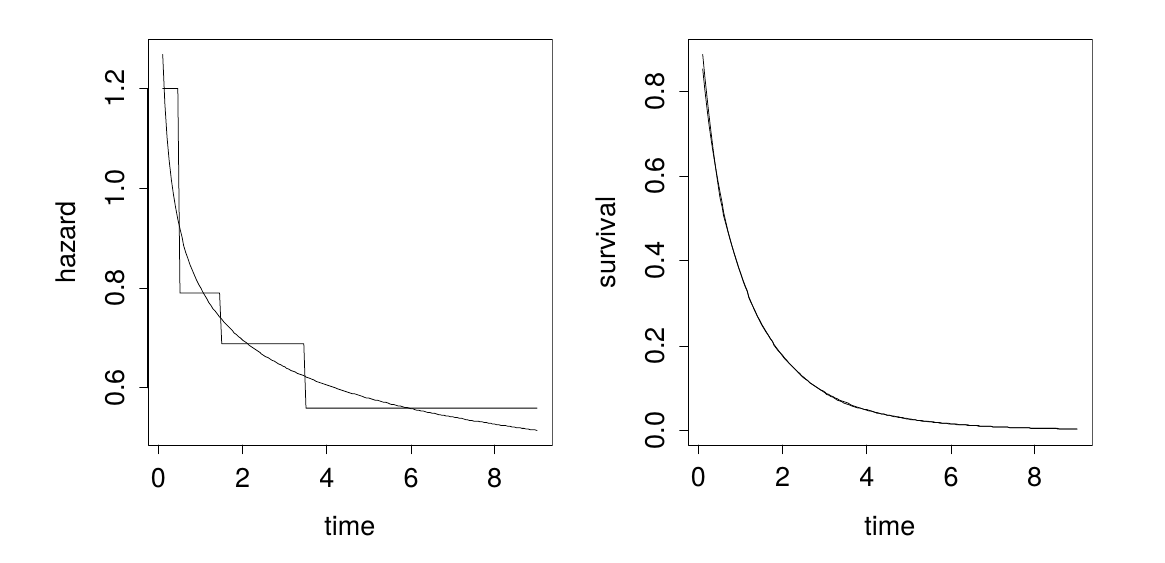
\includegraphics[height=0.2\textheight]{art/piecewise_exponential}
\caption{Piecewise Exponential aproximation of the Weibull distribution.}
\label{fig:piecewise_exponential}
\end{figure}


The piecewise-constant hazard model is very convenient to analyze under the proportional hazard assumption:
\begin{align}
	\hazard{x}{t} = \hazard{x_0}{t} e^{(x-x_0)'\beta} = h_j e^{(x-x_0)'\beta}.
\end{align}
There are $p+2J$ parameters to estimate.
This can be done directly using maximum likelihood, or by casting the problem as several separate Poisson regression problem. 
This has the benefit that the problem may be immediately solved with any statistical software suite, with existing numerical solvers.
We will currently not pursue this avenue, and refer the reader to the bibliographic notes.



\section{Collecting the pieces}
In this chapter we have seen the probabilistic reliability analysis, where we assumed components' reliabilities are known. 
We then proceeded to the statistical problem of estimating reliabilities from failure data.
We now glue collect these pieces to sketch a realistic analysis workflow, which would look roughly as follows:
\begin{enumerate}
\item Estimate reliability parameters by collecting component-wise failure data. Data is collected in a lab so that you may accelerate time and rescale to realistic operating conditions.
\item Perform the probabilistic analysis of the whole system using the estimated parameters.
\end{enumerate}



\begin{remark}[Interplay between probability and statistics]
There is obviously an interplay between the above stages:
In the statistical analysis, we want the least possible set of assumptions;
For the probabilistic analysis, the more we can assume, the more we can say about the system as a whole.
\end{remark}



\begin{remark}[What is a component?]
The notion of a ``system'' and a ``component'' is not well defined.
Indeed, for some purposes you may consider a system, as a component in a larger system.
For the statistical problem, a component is probably the smallest unit you can collect data on. At times, the smallest unit, may be the system as a whole.
\end{remark}




\section{Bibliographic Notes}
An light introductory discussion, may be found in \cite{nahmias_production_2015}. 
The probabilistic analysis in this text is adapted from \cite{aven_stochastic_1999}.
The seminal reference probably being \cite{barlow_mathematical_1965}.
The statistical analysis is adapted from German Rodriguez's Generalized-Linear-Models class notes\footnote{\url{http://data.princeton.edu/wws509/notes/c7.pdf}.} and \cite[Ch.8]{natrella_nist/sematech_2010}.
For more on the statistical analysis, see \cite{cox_analysis_1984}, \cite{kalbfleisch_statistical_2002}, or \cite{klein_survival_2005}.


% 